%  !TeX  root  =  user_guide.tex

\section{Модуль Оформление}

% когда переработка раздела будет завершена,
% раскоментируйте следующую строку:
% \updatedisclaimer

Модуль Оформление включает модули Знак авторского права, Указатель
<<Север-Юг>> и Масштабная линейка. Данные модули используются для
оформления карты использованием картографических элементов.

\subsection{Модуль Знак авторского права}

Название этого модуля вводит в заблуждение "--- вы можете добавить любой
произвольный текст на карту.

\begin{figure}[ht]
   \centering
   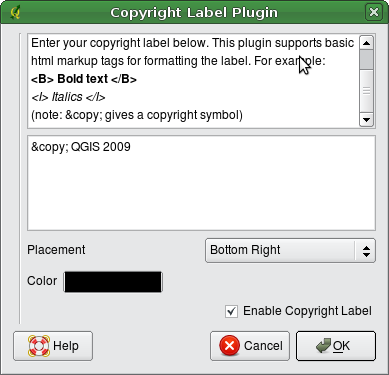
\includegraphics[clip=true, width=7cm]{copyright}
   \caption{Модуль Знака авторского права \wincaption}\label{fig:copyright}
\end{figure}

\begin{enumerate}
\item Убедитесь что модуль загружен
\item Выберите пункт меню \mainmenuopt{Модули} \arrow \dropmenuopt{Оформление}
\arrow \dropmenuopttwo{copyright_label}{Знак авторского права} или
используйте кнопку \toolbtntwo{copyright_label}{Знак авторского права}
на панели инструментов.
\item Введите текст который вы хотите разместить на карте. Вы можете
использовать язык разметки HTML как показано в примере.
\item Выберите местоположение надписи из раскрывающегося списка
\selectstring{{}Размещение}{Внизу справа}
\item Поставьте отметку в \checkbox{Включить знак авторского права}
\item Нажмите кнопку \button{OK}
\end{enumerate}

В примере выше (по умолчанию) символ авторского права с датой размещается
в нижнем правом угол поля карты.

\subsection{Модуль Указатель <<Север-Юг>>}

Модуль Указатель <<Север-Юг>> размещает на карте простую стрелку направленную
на север. В настоящее время для указателя доступен только один стиль. Вы
можете задать направление указателя или позволить QGIS определить его
автоматически. Если вы выберите вариант автоматического определения
направления, то QGIS предположит лучшее направление для указателя. Разметить
указатель возможно в любом из четырех углов поля карты.

\begin{figure}[ht]
   \centering
   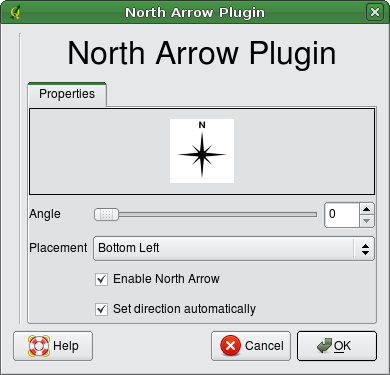
\includegraphics[clip=true, width=8cm]{north_arrow_dialog}
   \caption{Модуль Указатель <<Север-Юг>> \wincaption}\label{fig:north_arrow}
\end{figure}

\subsection{Модуль Масштабная линейка}
Модуль Масштабная линейка добавляет простую масштабную линейку на поле
карты. Вы можете определить стить и местоположение линейки аналогично
как для панели надписей.

QGIS поддерживает отображение масштаба только в тех же единицах измерения
что и карта. Т.\,е., если единица измерения на вашем слое метр, вы не
можете добавить Масштабную линейку в футах. Аналогично, если вы используете
десятичные градусы, то не можете создать Масштабную линейку с единицей
измерения метр.

Для добавления Масштабной линейки :

\begin{enumerate}
\item Выберите меню \mainmenuopt{Модули} \arrow \dropmenuopt{Офрмление}
\arrow \dropmenuopttwo{scale_bar}{Масштабная линейка} или используйте
кнопку \toolbtntwo{scale_bar}{Масштабная линейка} на панели инструментов.
\item Выберите вариант размещения в открывающемся списке
\selectstring{{}Размещение}{Внизу слева}
\item Выберите стиль из списка \selectstring{{}Стиль линейки}{Штрих вниз}
\item Выберите цвет линейки \selectcolor{{}Цвет линейки}{black} или используйте
базовый церный цвет
\item Установите размер линейки и надписи \selectnumber{{}Размер линейки}{30 градусов}
\item Поставьте отметку в \checkbox{Включить масштабную линейку}
\item Дополнительно можете выбрать автоматическое изменение размера для
округления показателя при изменении  размера поля карты \\
\checkbox{Автоматически изменять размер для округления показателя}
\item Нажмите кнопку \button{OK}
\end{enumerate}

\begin{figure}[ht]
   \centering
   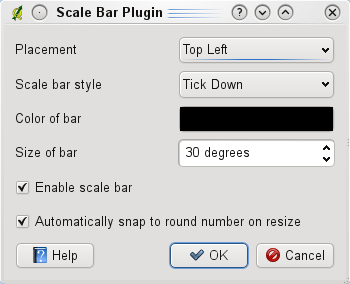
\includegraphics[clip=true, width=8cm]{scale_bar_dialog}
   \caption{Модуль масштабной линейки \wincaption}\label{fig:scale_bar}
\end{figure}

\begin{Tip}\caption{\textsc{Сохранение в проекте настроек модулей}}\index{настройки модулей}
Когда вы сохраняете проект в формате .qgs, любые изменения произведенные
с указателем <<Север-Юг>>, масштабной линейкой и знаком авторского права
так же будут сохранены и восстановлены при последующем открытии проекта.
\end{Tip}

\FloatBarrier
